\documentclass[12pt, a4paper]{article}  

\usepackage{csquotes}
\usepackage{etex} 
\usepackage{rotating}

%%%%%%%%%% Математика %%%%%%%%%%
\usepackage{amsmath,amsfonts,amssymb,amsthm,mathtools} 

%%%%%%%%%%%%%%%%%%%%%%%% Шрифты %%%%%%%%%%%%%%%%%%%%%%%%%%%%%%%%%
\usepackage{fontspec}       
\setmainfont{Arial}   

\defaultfontfeatures{Mapping=tex-text}

% why do we need \newfontfamily:
% http://tex.stackexchange.com/questions/91507/
\newfontfamily{\cyrillicfonttt}{Arial}
\newfontfamily{\cyrillicfont}{Arial}
\newfontfamily{\cyrillicfontsf}{Arial}

\usepackage{unicode-math}    
\setmathfont{Asana Math}    

\usepackage{polyglossia}      % Пакет, который позволяет подгружать русские буквы
\setdefaultlanguage{russian}  % Основной язык документа
\setotherlanguage{english}    % Второстепенный язык документа

%%%%%%%%%% Работа с картинками %%%%%%%%%
\usepackage{graphicx}                  % Для вставки рисунков
\usepackage{graphics}
\graphicspath{{images/}{pictures/}}    % можно указать папки с картинками
\usepackage{wrapfig}                   % Обтекание рисунков и таблиц текстом


%%%%%%%%%% Работа с таблицами %%%%%%%%%%
\usepackage{tabularx}            % новые типы колонок
\usepackage{tabulary}            % и ещё новые типы колонок
\usepackage{array}               % Дополнительная работа с таблицами
\usepackage{longtable}           % Длинные таблицы
\usepackage{multirow}            % Слияние строк в таблице
\usepackage{float}               % возможность позиционировать объекты в нужном месте
\usepackage{booktabs}            % таблицы как в книгах!
\renewcommand{\arraystretch}{1.3} % больше расстояние между строками

%%%%%%%%%% Графика и рисование %%%%%%%%%%
\usepackage{tikz, pgfplots}  % язык для рисования графики из latex'a
\usepackage{amscd}                  %Пакеты для рисования
\usepackage[matrix,arrow,curve]{xy} %комунитативных диаграмм

%%%%%%%%%% Теоремы %%%%%%%%%%
\theoremstyle{plain}              % Это стиль по умолчанию.  Есть другие стили. 
\newtheorem{theorem}{Теорема}[section]
\newtheorem{result}{Следствие}[theorem]
% счётчик подчиняется теоремному, нумерация идёт по главам согласованно между собой

%%%%%%%%% Свои команды %%%%%%%%%%
\usepackage{etoolbox}    % логические операторы для своих макросов


% Все свои команды лучше всего определять не по ходу текста, как это сделано в этом документе, а в преамбуле!


\usepackage{indentfirst}
\setkeys{russian}{babelshorthands=true}

\DeclareMathOperator{\Corr}{Corr}
\DeclareMathOperator{\Var}{Var}

\title{Домашняя работа № 3}
\date{\today}

\begin{document}

\maketitle

\section{Задание 1 (математические операторы)}
В преамбуле можно сздать такие математические операторы как $\Var$ и $\Corr$

\section{Задание 2 (сигма)}
\newcommand{\s}{\ensuremath{\sigma}}
\s - алгебра — алгебра множеств, замкнутая относительно операции счётного объединения.

\section{Задание 3 (последовательность)}
\newcommand{\n}{\ensuremath{x_1	\ldots	x_n}}
\[ \n \]

\section{Задание 4 (последовательности }
\newcommand{\nn}[2]{\ensuremath{x_{#1} \ldots x_{#2}}}
\[ \nn{a}{z} \]
\[ \nn{1}{6} \]
\[ \nn{(a,b)}{(c,d)} \]

\section{Задание 5 (список)}
\begin{itemize}
\newcommand{\itemcolor}[1]{\renewcommand{\makelabel}[1]{\color{#1}\hfil ##1}}
\itemcolor{blue}
\item  Первый пункт 
\item  Второй пункт 
\item  Третий пункт 
\end{itemize}

\section{Задание 6 (предел)}
\newcommand{\llim}[3]{\ensuremath{\lim\limits_{{#1} \to {#2}} {#3}}}

\[ \llim{n}{\infty}{\frac{n+1}{n}} \]
\[ \llim{n}{\infty}{\left(1+\frac{1}{n}\right)^n = e} \]

\section{Задание 7 (нумерация рисунков)}
\setcounter{figure}{0}
\renewcommand{\thefigure}{\arabic{section}.\arabic{figure}}

\begin{figure}[H]
\begin{center}
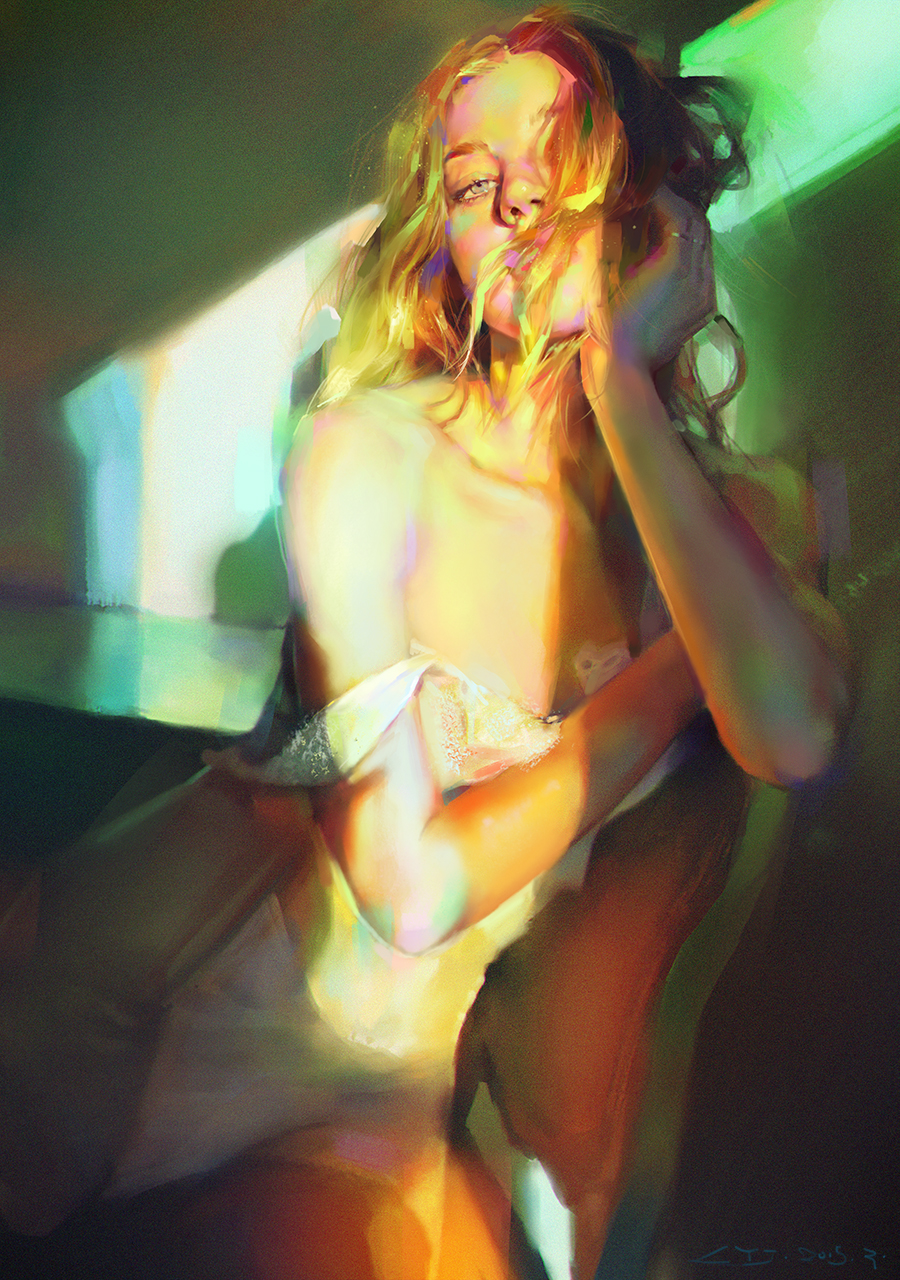
\includegraphics[scale=0.2]{y1.jpg}
\end{center}
\caption{Художник - Yanjun Cheng}
\end{figure}

\begin{figure}[H]
\begin{center}
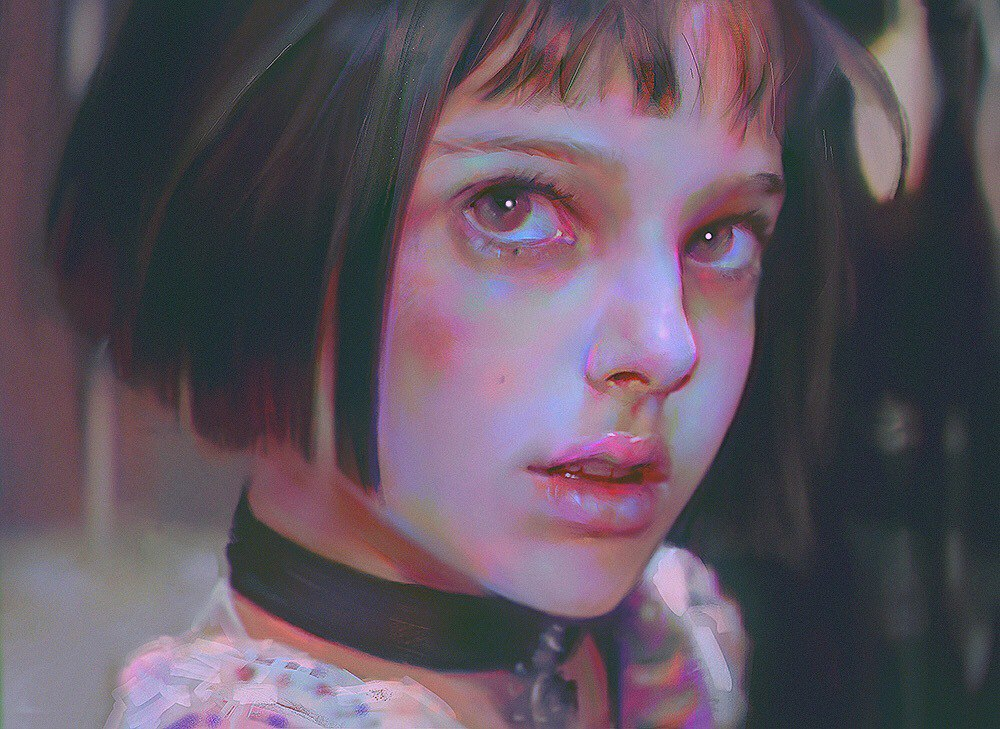
\includegraphics{y2.jpg}
\end{center}
\caption{Художник - Yanjun Cheng}
\end{figure}

\section{Задание 8 (нумерация формул)}
\setcounter{equation}{0}
\renewcommand{\theequation}{Eq.(\arabic{equation})}

\begin{equation}
\sigma_{\hat \beta_1} = \frac {Var((x_i - \mu_x)\cdot u_i)}{n \cdot (Var (x_i))^2}
\end{equation}

\begin{equation}
\int_0^{\infty} e^{-x^2} dx = \frac{\pi}{2} 
\end{equation}

\section{Задание 9}
\newcounter{i}
\newbool{answers}
\booltrue{answers}

\newcommand{\yesno}[3][]{
\addtocounter{i}{1}
\textcolor{cyan}{\textbf{Данетка \arabic{i}}}
\ifbool{answers}{\begin{center}\textbf{<<#1>>}\end{center}}{ }
\begin{displayquote}
#2\\
\end{displayquote}
\textbf{Ответ:} \begin{turn}{180}\parbox{\linewidth}{\textit{#3}}\end{turn}\\\\}

\yesno[Пятёрка за экзамен]{Экзамен в военно-морском училище. Курсант вытянул билет и сел готовиться. Вдруг, ни с того ни с сего, он встаёт с места и подходит к профессору с зачётной книжкой. Тот, не раздумывая, ставит ему «пять». Как такое возможно?}{Преподаватель, используя азбуку морзе, простучал по столу карандашом сообщение: «Первый, кто расшифрует это послание, пусть подойдёт ко мне и сразу, без сдачи экзамена получит оценку отлично». Студент расшифровал сообщение и получил заслуженную пятёрку.}

\yesno[Наществие котов]{Один человек уехал в отпуск и попросил друга присмотреть за котом. Через неделю в квартире бегали уже 8 взрослых котов. Откуда они взялись?}{На следующий день кот убежал, и человеку пришлось дать объявление о пропаже. Поскольку он сам ещё не очень хорошо знал кота, ему пришлось оставлять у себя всех похожих котов, которых ему приносили. И ждать приезда друга, который должен был опознать своего питомца.}

\yesno[Странные девушки]{Рядом стоят три девушки, две из них расстроены, одна счастлива. Счастливая девушка плачет, а расстроенные – улыбаются. Что происходит?}{Конкурс красоты. Проигравшие девушки улыбаются, победительница плачет от счастья.}

\end{document}